% vim: set spell spelllang=es syntax=tex :

\documentclass[11pt,a4paper,spanish]{beamer}

\usepackage[spanish]{babel}

\usepackage[utf8]{inputenc}

\usepackage{graphicx}

\usepackage{subcaption} %Para Subfigure

\usepackage{caption} %Para captions en las figuras sin prefijo

\usepackage{ccicons}

\usepackage{url}

\usepackage{babelbib}

\usefonttheme{serif}

\setlength{\parskip}{1.5mm}

\newcommand{\codeword}[1]{\mbox{\texttt{\textcolor{blue}{#1}}}}

\usetheme{Rochester}
\usecolortheme{whale}

%\usetheme{Warsaw}

\beamertemplatenavigationsymbolsempty

\setbeamertemplate{background canvas}{
    \raisebox{-0.99\paperheight}[0pt][0pt]{
        \makebox[\paperwidth]{
            \null
            \hspace{-1em}
            \includegraphics[width=0.09\paperwidth]{logos/fai.pdf}
            \hspace{0.8\paperwidth}
            %\hfill
            \hspace{-1em}
            \includegraphics[width=0.09\paperwidth]{logos/uncoma.pdf}
            }
    }
}

\title{\textbf{Introducción a la\\
Administración de sistemas}}

\author{}

\date{}

\defbeamertemplate{footline}{centered page number}
{
    \hspace*{\fill}
    \usebeamercolor[fg]{blue}
    \usebeamerfont{page number in head/foot}
    \insertpagenumber\,/\,\insertpresentationendpage
    \hspace*{\fill}\vskip2pt
}
\setbeamertemplate{footline}[centered page number]

\begin{document}

\begin{frame}[noframenumbering]

    \maketitle
    \centering
    \vspace{-8em}~
    \begin{figure}
    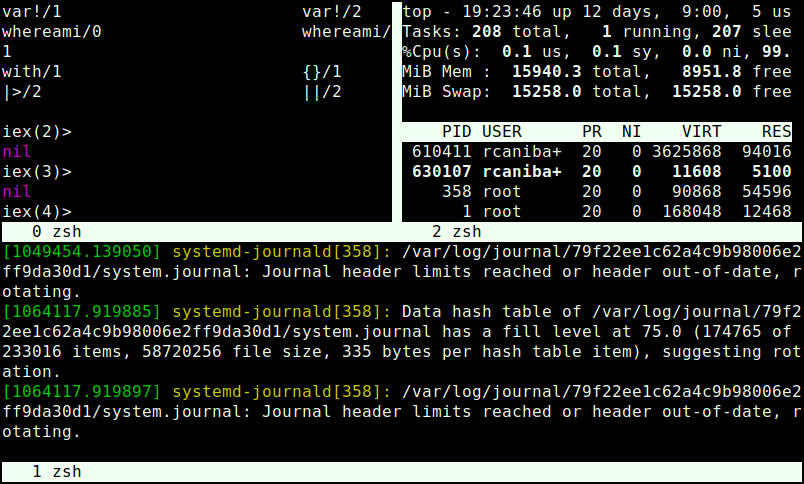
\includegraphics[height=0.55\textheight]{img/screen.pdf}
    \end{figure}

\end{frame}

\begin{frame}

    \frametitle{Temario}

\begin{itemize}

    \item ¿Qué tareas realiza un administrador de sistemas?
    \item ¿Qué método nos permite una administración medianamente homogénea?
        \begin{itemize}
            \item Sistemas de tipo \texttt{UNIX}.
            \item ¿Qué es un shell?
            \item Interfaz por linea de comandos: el \emph{UNIX Shell}.
            \item \emph{Secure Shell}: \codeword{ssh}.
            \item Editor \codeword{Vim}.
        \end{itemize}

\end{itemize}

\end{frame}

\begin{frame}

    \frametitle{Administración de sistemas}
    \framesubtitle{¿Qué es administrar un sistema?}

\begin{itemize}
    \item Administración de recursos:
        \begin{itemize}
            \item Redes.
            \item Almacenamiento.
            \item Bases de datos.
            \item Impresoras.
            \item \emph{etc.}
        \end{itemize}
    \item Seguridad y protección:
        \begin{itemize}
            \item Usuarios.
            \item Detección de anomalías.
            \item Copias de respaldo.
            \item \emph{etc.}
        \end{itemize}
    \item Automatización de tareas.
    \item Documentación.
    \item \emph{etc.}, \emph{etc.}, \emph{etc.}...
\end{itemize}

\end{frame}

\begin{frame}

    \frametitle{Administración de sistemas}
    \framesubtitle{¿Qué método nos permite una administración medianamente
    homogénea?}

    \begin{figure}
    \centering
    \includegraphics[height=0.80\textheight]{img/jurassicPark.png}
        \captionsetup{textfont=tiny,labelformat=empty}
        \caption{``\emph{It is a \texttt{UNIX} system! I know this!}''\\
        Jurassic Park (1993)}
    \end{figure}
\end{frame}

\begin{frame}

    \frametitle{Administración de sistemas}
    \framesubtitle{¿Qué método nos permite una administración medianamente
    homogénea?}

    Los sistemas \texttt{UNIX}, \texttt{POSIX}, y
    \texttt{UNIX-like}\footnote{\texttt{UNIX} es una marca registrada, y el
    uso del termino \texttt{UNIX-like} no esta aprobado oficialmente. Sin
    embargo, su uso esta fuertemente extendido y arraigado en el léxico
    informático.} permiten una administración y uso uniforme de distintos
    sistemas de computo. Si bien hay diferencias, a grandes rasgos comparten:

\begin{itemize}
    \item Jerarquía de directorios.
    \item Software.
    \item Configuración.
    \item La \emph{filosofía \texttt{UNIX}}:
        \begin{itemize}
            \item Cada programa hace una cosa bien.
            \item Los programas deben trabajar juntos.
            \item Los programas manipulas flujos de texto, esa es la interfaz
                universal.
        \end{itemize}
\end{itemize}

\end{frame}

\begin{frame}
    \frametitle{Administración de sistemas}
    \framesubtitle{Genealogía de los sistemas \texttt{UNIX-like}}

    \begin{figure}
    \centering
    \includegraphics[height=0.9\textheight]{img/unixTimeline.pdf}
        \captionsetup{textfont=tiny,labelformat=empty,justification=centering}
        \caption{\ccPublicDomain\cite{unixTimeline}}
    \end{figure}

\end{frame}

\begin{frame}

    \frametitle{Administración de sistemas}
    \framesubtitle{Definición \emph{shell}}

    El \emph{Shell} de un sistema es un proceso que funciona de interfaz
    entre el usuario y la computadora. Puede ser de solo texto o gráfico.

    \begin{figure}
    \centering
    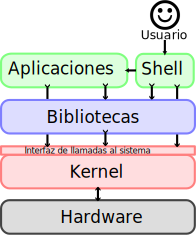
\includegraphics[height=0.65\textheight]{img/os.pdf}
        \captionsetup{textfont=tiny,labelformat=empty,justification=centering}
        \caption{}
    \end{figure}

\end{frame}

\begin{frame}

    \frametitle{Administración de sistemas}
    \framesubtitle{\emph{Shell} gráfico}

    \begin{figure}
    \centering
    \includegraphics[height=0.8\textheight]{img/xwinsys.png}
        \captionsetup{textfont=tiny,labelformat=empty,justification=centering}
        \caption{(MIT)\cite{xwinsys}}
    \end{figure}

\end{frame}

\begin{frame}

    \frametitle{Interfaz por linea de comandos}
    \framesubtitle{El \texttt{UNIX} \emph{Shell}}

    Es un interprete por linea de comandos común a todos los sistemas de tipo
    \texttt{UNIX}.
    \begin{itemize}
        \item Interfaz de usuario y lenguaje de \emph{scripting}.
        \item Variantes: \emph{sh}, \emph{BASH}, \emph{zsh}, \emph{bussybox},
            etc.
    \item Bajo consumo de recursos.
    \end{itemize}

    \begin{figure}
    \centering
    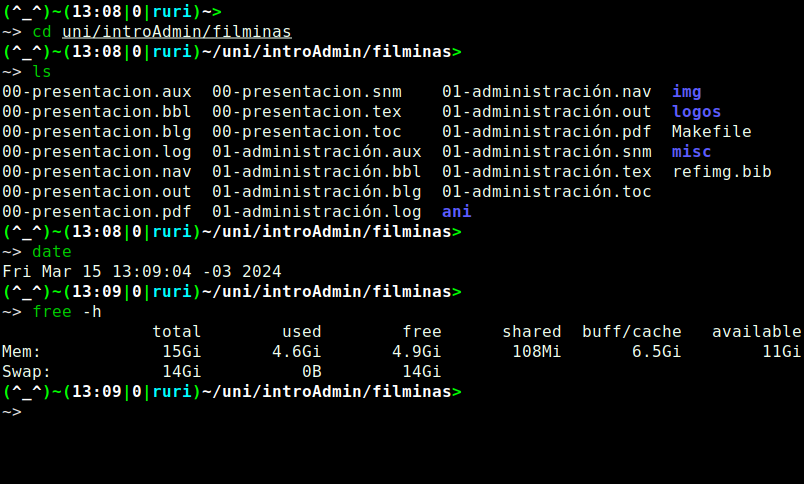
\includegraphics[height=0.4\textheight]{img/unixShell.pdf}
    \end{figure}

\end{frame}

\begin{frame}

    \frametitle{Interfaz por linea de comandos}
    \framesubtitle{\emph{Secure Shell}: \codeword{ssh}}
    
    \codeword{SSH} es un protocolo seguro de conexión remota. Su uso más
    común es ejecutar un \codeword{shell} remoto en una terminal local.

        \codeword{ssh \$USER@aula-ssh.fi.uncoma.edu.ar -p 60173}
        \begin{itemize}
            \item[] \tiny{\emph{(Remplazar \codeword{\$USER} por su usuario
                de laboratorio)}}
        \end{itemize}

    \begin{figure}
    \centering
    \includegraphics[height=0.6\textheight]{img/ssh.png}
        \captionsetup{textfont=tiny,labelformat=empty}
        \caption{Fuente desconocida}
    \end{figure}

\end{frame}

\begin{frame}

    \frametitle{Interfaz por linea de comandos}
    \framesubtitle{Editor \texttt{Vim}}
    
    \codeword{Vim} (de \texttt{vi} \emph{improved}) es un editor modal para
    terminales de texto altamente configurable que esta pre instalado en la
    gran mayoría de los sistemas de tipo \texttt{UNIX}\footnote{sino,
    posiblemente este instalado su predecesor \codeword{vi}}. Fue diseñado
    especialmente para terminales con conexiones lentas, por lo que es ideal
    para ser utilizado por \codeword{SSH}.

    \begin{figure}
    \centering
    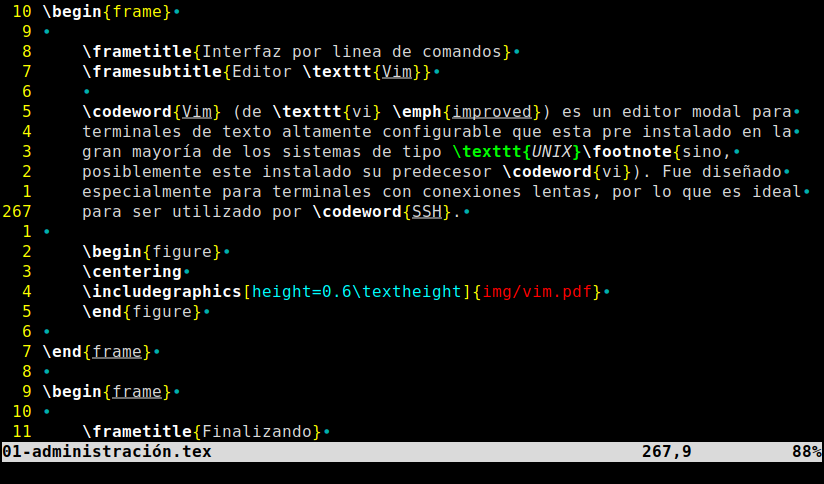
\includegraphics[height=0.5\textheight]{img/vim.pdf}
    \end{figure}

\end{frame}

\begin{frame}

    \frametitle{Finalizando}

\begin{itemize}

    \item ¿Qué tareas realiza un administrador de sistemas?
    \item ¿Qué método nos permite una administración medianamente homogénea?
        \begin{itemize}
            \item Sistemas de tipo \texttt{UNIX}.
            \item ¿Qué es un shell?
            \item Interfaz por linea de comandos: el \emph{UNIX Shell}.
            \item \emph{Secure Shell}: \codeword{ssh}.
            \item Editor \codeword{Vim}.
        \end{itemize}

\end{itemize}

\end{frame}

\begin{frame}

\title{¿Consultas?}
\maketitle

\end{frame}

\newcounter{lastPage}
\setcounter{lastPage}{\number\value{page}}

\begin{frame}%[allowframebreaks]

\frametitle{Atribuciones}

\bibliographystyle{abbrv}
\setbeamertemplate{bibliography item}{\insertbiblabel}
\tiny
\bibliography{refimg}
\end{frame}

\setcounter{page}{\number\value{lastPage}}

\end{document}
